\documentclass[11pt]{article}
\usepackage{graphicx}
\usepackage{float}

\begin{document}

% TITLE:
\title{Movie Web Scraper}
\date{}
\maketitle
% %%%%%%%%%%%%%%%%%%
\begin{abstract}\noindent Report about design and development of a Web scraper, a Python bot, thought for retrieving data to populate and update movie info collections on Movienator MongoDB document-oriented database . 

% END CONTENT ABS------------------------------------------
\end{abstract}


% %%%%%%%%%%%%%%%%%%%%%%%%%%%%%%%%%%%%%%%%%%%%%%%%%%%%%%%%%%
% %%%%%%%%%%%%%%%%%%%%%%%%%%%%%%%%%%%%%%%%%%%%%%%%%%%%%%%%%%
% BODY OF THE DOCUMENT
% %%%%%%%%%%%%%%%%%%%%%%%%%%%%%%%%%%%%%%%%%%%%%%%%%%%%%%%%%%
% %%%%%%%%%%%%%%%%%%%%%%%%%%%%%%%%%%%%%%%%%%%%%%%%%%%%%%%%%%

% --------------------
\section{Scope of Scraper Bot}
% --------------------
The aim of this bot, developed in Python (3.7) language, is to solve the problem of lack of data, indeed Movienator app needs a lot of movie information and details to work sensibly, so the scraper works providing from several sources (MyMovies, IMDb ..) all types of data required, according to the ETL ("Extract-Transform-Load") paradigm.\\\newline
We can identify two main uses of the scraper, as follow:
\begin{enumerate}
    \item Find new movies and related details; a movie is "new" if not already stored as a MongoDB collection.
    \item Update movies with most recent data, this operation is carried out periodically.
\end{enumerate}
Below are listed all the attributes collected by the scraper for each movie:\newline
\begin{itemize}
    \item movie title;
    \item movie genre;
    \item URL to movie poster;
    \item movie description;
    \item public release date;
    \item aggregate rate of external source;
    \item extra attributes (storyline, tagline, production country, budget ..)
\end{itemize}

% --------------------
\newpage
\section{Software design according to ETL model}
% --------------------
\subsection{Data extraction}
The very first step is data extraction, made possible by sequential HTTP requests (performed by Requests module), followed by the utilization of Beautiful Soup, a Python library for pulling data out of HTML and XML files.
Data, among different http responses, are retrieved by a JSON-LD tag, contained within html body of every single movie page.
\begin{figure}[H]
    \centering
        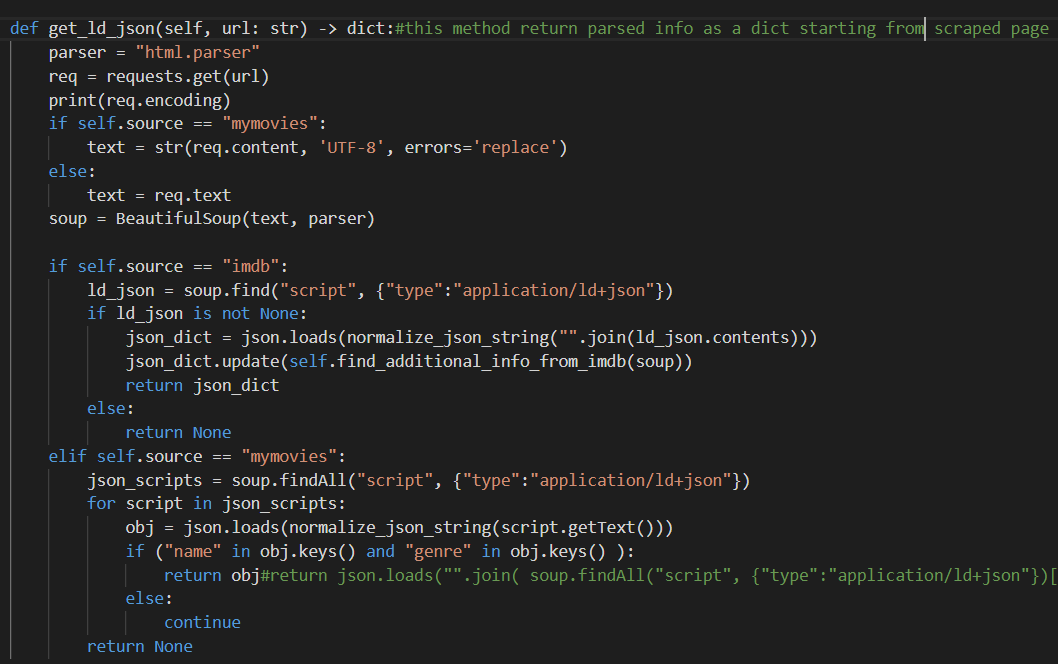
\includegraphics[width=1.0\textwidth]{figures/codepic/f1.png}
    \caption{Data extraction, performed by Requests and BeautifulSoup methods}
    \label{fig:1}
\end{figure}
\noindent Web indexing is made agile through two separate techniques:
\begin{enumerate}
    \item Across IMDb pages, every movie page is uniquely identified by imdb\_id, exploiting a standard URL format, "\emph{https://www.imdb.com/title/ttxxxxxxx/}", where \emph{"xxxxxxx"} is the integer id to locate the source.
    \item Exploiting MyMovies Web API, it's possible to find movies URL starting from their titles; "\emph{https://www.mymovies.it/ricerca/ricerca.php?limit=true\&q=yyyyyyy}", this is the query format, where the real argument (passed by GET method) is actually just one, \emph{"q"} and \emph{"yyyyyyy"} rapresents movie title.
\end{enumerate}
\newpage\noindent
% --------------------
\subsection{Data transformation}
All the input data, retrieved from Web, are parsed into Python dictionaries, exploiting json library methods applied to deserialized data content, which is obtained by the \emph{"soup"} in the previous phase.

\begin{figure}[H]
    \centering
        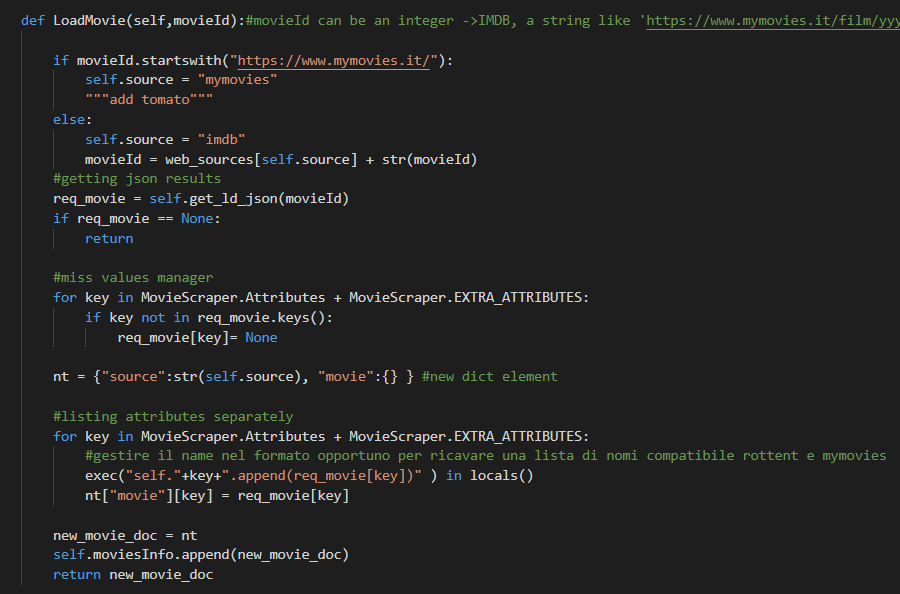
\includegraphics[width=1.0\textwidth]{figures/codepic/f2.png}
    \caption{Data parsing and standardization}
    \label{fig:1}
\end{figure}
% --------------------
\noindent In the figure above (Fig.2) we can look at the code that performs a first processing of data, retrieved by the dictionary resulting from the deserialization of the json content. Missing features are converted in properties with \emph{None} as a value, the objetive is to deal with standard format dictionaries, solving the problem of heterogeneous data sources.\newpage

\subsection{Data loading: updating the database}
New scraped data, both for features update and addition, once parsed, are stored on MongoDB server by means of PyMongo API for Mongo DBMS. BSON is the standard format used to store documents and make remote procedure calls in MongoDB, luckily python dictionares are directly mapped to BSON type as object and vice versa, so serialization (writings to Mongo) and deserialization (readings from Mongo) processes are easily managed.
\begin{figure}[H]
    \centering
        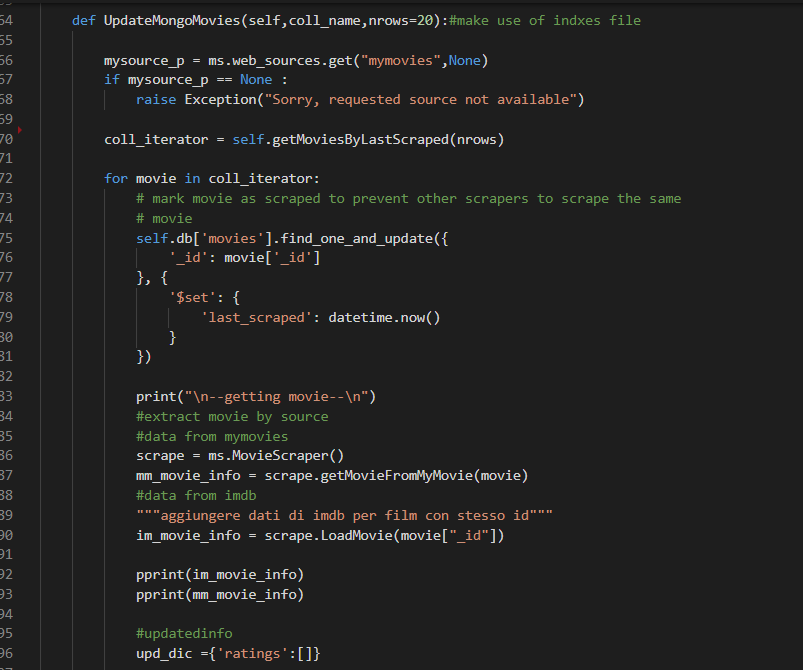
\includegraphics[width=1.0\textwidth]{figures/codepic/f31.png}
    \caption{Data extraction (performed by Requests and BeautifulSoup libs)}
    \label{fig:1}
\end{figure}
\noindent In order to perform optimized update operations, a \emph{last\_scraped} attribute is added (and modified) every time an update operation is executed from the script: this attribute is just an index to keep trace of the movies that were not updated longer. The code above (Fig.3) shows how to process consecutive movies, getting them by \emph{self.getMoviesByLastScraped} method and proceeding on integrating scraped data.
\newpage
% --------------------
\begin{figure}[H]
    \centering
        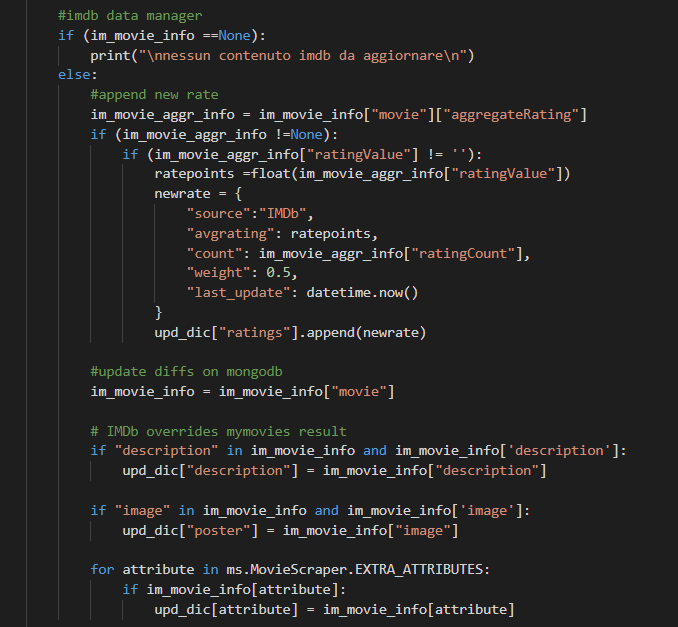
\includegraphics[scale=.55]{figures/codepic/f4.png}
    \caption{IMDb data integration}
    \label{fig:1}
    \centering
        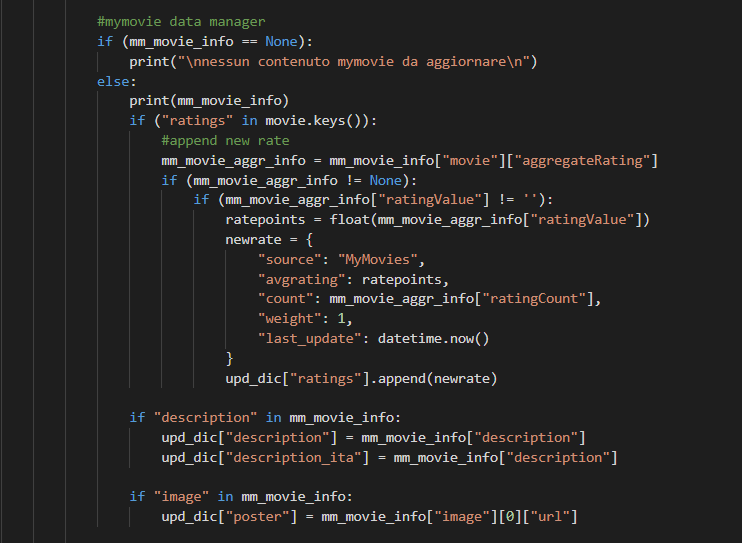
\includegraphics[scale=.5]{figures/codepic/f3.png}
    \caption{MyMovies data integration}
    \label{fig:1}
\end{figure}
% --------------------
\newpage\noindent
Some types of information, like \emph{total\_rating} feature, need to be computed incrementally, merging each time new scraped data coming from both MyMovies and IMDb.\\In order to interact with Mongo database we exploited several methods from PyMongo module, as:
\begin{itemize}
    \item findOne()
    \item updateOne()
    \item find\_one\_and\_update()
    \item bulk\_write()
\end{itemize}
All these methods take dictionaries as argument, with the exception of \emph{bulk\_write}, that is used for increasing write throughput.
\begin{figure}[H]
    \centering
        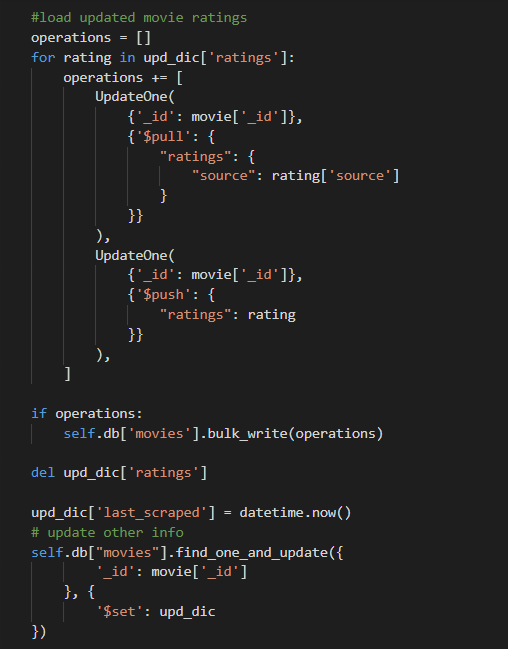
\includegraphics[scale=.65]{figures/codepic/f5.png}
    \caption{bulk update operations}
    \label{fig:1}
\end{figure}
% --------------------
\end{document}